\documentclass{beamer}
\usepackage{graphicx}

\title{Deep G-Buffers for stable Global Illumination Approximation}
\author{Ferit Tohidi Far}
\usetheme{Frankfurt}

\begin{document}
	\maketitle

	\begin{frame}
		\frametitle{Content}
		\begin{itemize}
			\item Global illumination
				\begin{itemize}
					\item Pathtracing
					\item Visual effects
					\item Radiosity
					\item Inefficiency
				\end{itemize}
			\item Traditional rendering
				\begin{itemize}
					\item Forward rendering
					\item Deferred rendering
				\end{itemize}
			\item Deep G-Buffers)
				\begin{itemize}
					\item Benefits
					\item Generating 2-layer deep g-buffer
					\item Global illumination approximation
				\end{itemize}
		\end{itemize}
	\end{frame}

	\begin{frame}
		\frametitle{Global illumination}
		\begin{itemize}
			\item lighting of a scene
			\item direct \textbf{and indirect} light is considered
			\item causes visual effects that convey realism
			\item most popular method is pathtracing
		\end{itemize}
	\end{frame}

	\begin{frame}
		\frametitle{Pathtracing}
		\begin{itemize}
			\item monte-carlo simulation
			\item send camera ray through each pixel
			\item allow ray to reflect \textbf{diffusely or specularly}
			\item trace it back to a light source
			\item if a light source was hit, the pixel is colored (albedo of hit-object)
			\item else the pixel is black (in shadow)
			\item each pixel is sampled thousands of times, then averaged
		\end{itemize}
	\end{frame}

	\begin{frame}
		\frametitle{Visual effects}
		\begin{center}
			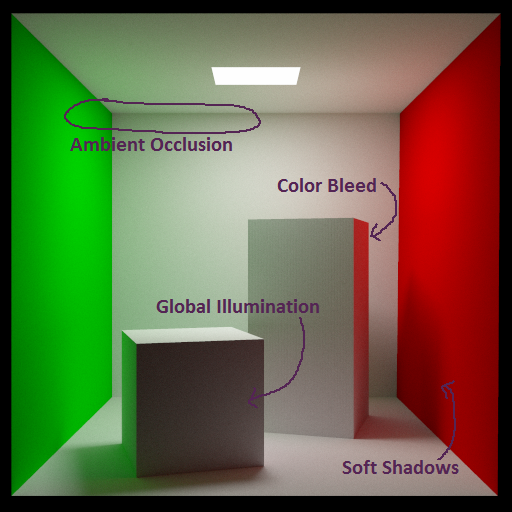
\includegraphics[width=.7\textwidth]{img/visual_effects.png}
		\end{center}
	\end{frame}

	\begin{frame}
		\frametitle{Radiosity}
		\begin{itemize}
			\item scene is divided into patches
			\item each patch is a light receiver and emitter 
			\item initialize scene with at least one patch that emits non-zero amount of light
			\item iteratively update receivance and emitance of each patch
			\item \textbf{purely diffuse global illumination}
		\end{itemize}

		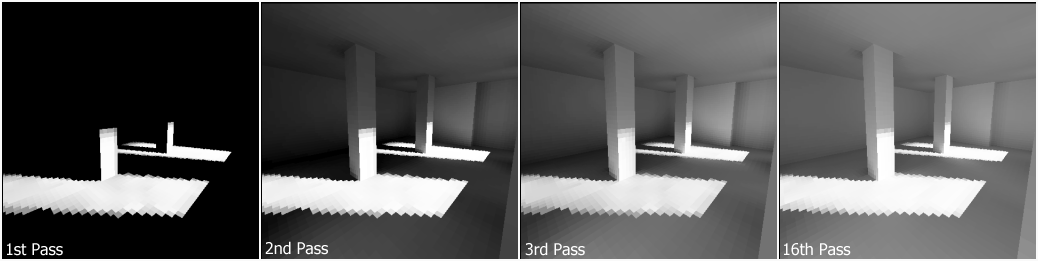
\includegraphics[width=\textwidth]{img/radiosity.png}
	\end{frame}

	\begin{frame}
		\frametitle{Inefficiency}
		\begin{itemize}
			\item pathtracing 
				\begin{itemize}
					\item computes multiple ray bounces
					\item requires thousands of samples (probably more) 
				\end{itemize}
			\item radiosity
				\begin{itemize}
					\item needs large amount of patches for good results
					\item has to be recomputed if an object moves
				\end{itemize}
			\item both cannot be computed in real-time (yet)
		\end{itemize}
	\end{frame}

	\begin{frame}
		\frametitle{Traditional rendering}
		\begin{itemize}
			\item rasterization
			\item way easier to compute than raytracing
			\item interactive framerates
			\item trade-off: not as realistic
			\item requires techniques to simulate visual effects
		\end{itemize}
	\end{frame}

	\begin{frame}
		\frametitle{Forward rendering}
		\begin{itemize}
			\item computes lighting in a single pass:
				\begin{itemize}
					\item for each fragment compute lighting
					\item do z-test
					\item render to frame-buffer or discard accordingly
					\item render frame-buffer to screen
				\end{itemize}
			\item computes lighting for fragment regardless if visible or not
		\end{itemize}
	\end{frame}

	\begin{frame}
		\frametitle{Deferred rendering}
		\begin{itemize}
			\item computes geometry (stored in g-buffer) in first pass:
				\begin{itemize}
					\item albedo-buffer
					\item normal-buffer
					\item z-buffer
				\end{itemize}
			\item render g-buffer to texture-buffer
			\item compute lighting in second pass:
				\begin{itemize}
					\item read frontmost scene geometry from g-buffer
					\item compute lighting
					\item render to screen
				\end{itemize}
			\item only computes lighting for visible fragments
		\end{itemize}
	\end{frame}

	\begin{frame}
		\frametitle{Deep G-Buffers}
		\begin{itemize}
			\item generate 2-layer deep g-buffer with depth-peeling or oracle
			\item enforce minimum depth separation
			\item consider second layer for visual effects
		\end{itemize}
	\end{frame}	

	\begin{frame}
		\frametitle{Generating a 2-layer deep g-buffer (depth-peeling)}
		\begin{itemize}
			\item \textbf{depth-peeling method}
			\item collect first layer g-buffer as usual
			\item compute second layer g-buffer by stripping the first layer
			\item takes two passes over scene geometry
		\end{itemize}
	\end{frame}	

	\begin{frame}
		\frametitle{Generating a 2-layer deep g-buffer (oracle)}
		\begin{itemize}
			\item \textbf{oracle method}
			\item collect first layer g-buffer as usual
			\item compute second layer g-buffer by stripping the first layer
			\item takes two passes over scene geometry
		\end{itemize}
	\end{frame}	

	\begin{frame}
		\frametitle{Results}
		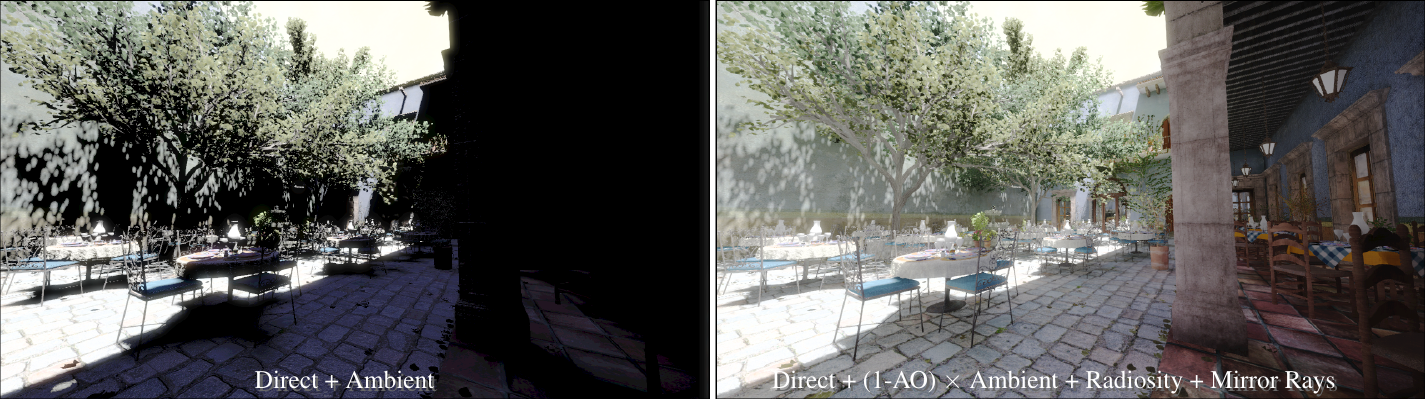
\includegraphics[width=\textwidth]{img/deep_g_buffer_render.png}
		\begin{itemize}
			\item 1920x1080 resolution
			\item rendered using NVIDIA GeForce 980
			\item in 10.8ms (92 FPS)
			\item looks good
		\end{itemize}
	\end{frame}

\end{document}